\documentclass{article}

\usepackage{amsmath,amssymb}
\usepackage{tikz}
\usepackage{pgfplots}
\usepackage{xcolor}
\usepackage{colortbl}
\usepackage[left=2.1cm,right=3.1cm,bottom=3cm,footskip=0.75cm,headsep=0.5cm]{geometry}
\usepackage{enumerate}
\usepackage{enumitem}
\usepackage{marvosym}
\usepackage{tabularx}
\usepackage[amsmath,thmmarks,standard]{ntheorem}
\usepackage{mathtools}
\usepackage{longtable}

\usepackage[utf8]{inputenc}

\renewcommand*{\arraystretch}{1.4}
\newcommand{\E}{\mathbb{E}}

\newcolumntype{L}[1]{>{\raggedright\arraybackslash}p{#1}}
\newcolumntype{R}[1]{>{\raggedleft\arraybackslash}p{#1}}
\newcolumntype{C}[1]{>{\centering\let\newline\\\arraybackslash\hspace{0pt}}m{#1}}

\DeclareMathOperator{\tr}{tr}
\DeclareMathOperator{\Var}{Var}
\DeclareMathOperator{\Cov}{Cov}
\renewcommand{\E}{\mathbb{E}}

\newtheorem{thm}{Theorem}
\newtheorem{lem}{Lemma}

\title{\textbf{Einführung in die Logistik, Übung 6}}
\author{\textsc{Henry Haustein}}
\date{}

\begin{document}
	\maketitle
	
	\section*{Aufgabe 19}
	Sweep-Algorithmus
	\begin{center}
		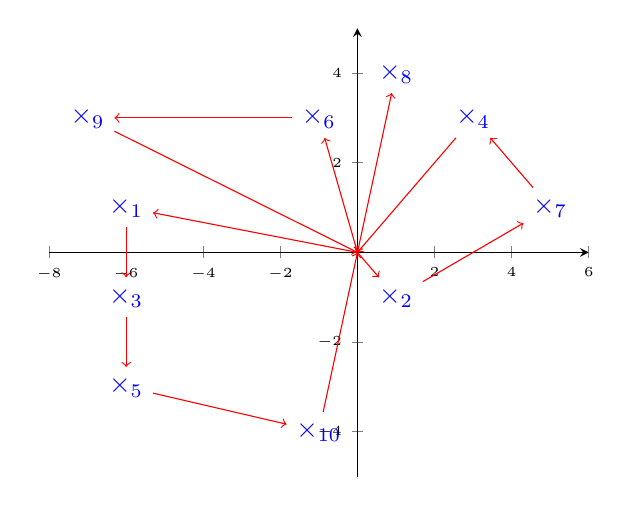
\begin{tikzpicture}
			\begin{axis}[
				xmin=-8, xmax=6,
				ymin=-5, ymax=5,
				samples=400,
				axis x line=middle,
				axis y line=middle,
				xticklabel style={font=\tiny},
				yticklabel style={font=\tiny}
				]
				
				\node[blue] at (axis cs: -6,1) (1) {$\times_1$};
				\node[blue] at (axis cs: 1,-1) (2) {$\times_2$};
				\node[blue] at (axis cs: -6,-1) (3) {$\times_3$};
				\node[blue] at (axis cs: 3,3) (4) {$\times_4$};
				\node[blue] at (axis cs: -6,-3) (5) {$\times_5$};
				\node[blue] at (axis cs: -1,3) (6) {$\times_6$};
				\node[blue] at (axis cs: 5,1) (7) {$\times_7$};
				\node[blue] at (axis cs: 1,4) (8) {$\times_8$};
				\node[blue] at (axis cs: -7,3) (9) {$\times_9$};
				\node[blue] at (axis cs: -1,-4) (10) {$\times_{10}$};
				
				\draw[->,red] (axis cs: 0,0) -- (6);
				\draw[->,red] (6) -- (9);
				\draw[->,red] (9) -- (axis cs: 0,0);
				\draw[->,red] (axis cs: 0,0) -- (1);
				\draw[->,red] (1) -- (3);
				\draw[->,red] (3) -- (5);
				\draw[->,red] (5) -- (10);
				\draw[->,red] (10) -- (axis cs: 0,0);
				\draw[->,red] (axis cs: 0,0) -- (2);
				\draw[->,red] (2) -- (7);
				\draw[->,red] (7) -- (4);
				\draw[->,red] (4) -- (axis cs: 0,0);
				\draw[<->,red] (axis cs: 0,0) -- (8);
			\end{axis}
		\end{tikzpicture}
	\end{center}
	Touren:
	\begin{itemize}
		\item Lager - 6 - 9 - Lager
		\item Lager - 1 - 3 - 5 - 10 - Lager
		\item Lager - 2 - 7 - 4 - Lager
		\item Lager - 8 - Lager
	\end{itemize}

	\section*{Aufgabe 20}
	\begin{enumerate}[label=(\alph*)]
		\item Erzeugnisbaum
		\begin{center}
			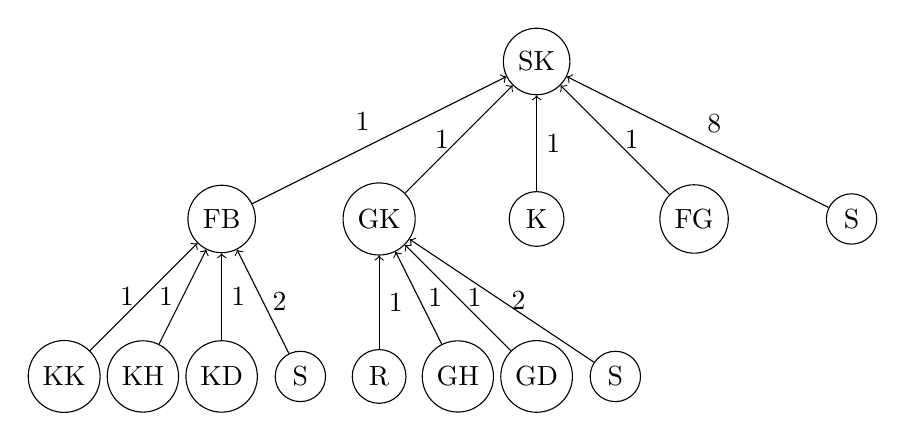
\begin{tikzpicture}
				\node[circle,draw=black, fill=white] (SK) at (0,0) {SK};
				
				\node[circle,draw=black, fill=white] (FB) at (-4,-2) {FB};
				\node[circle,draw=black, fill=white] (GK) at (-2,-2) {GK};
				\node[circle,draw=black, fill=white] (K) at (0,-2) {K};
				\node[circle,draw=black, fill=white] (FG) at (2,-2) {FG};
				\node[circle,draw=black, fill=white] (S1) at (4,-2) {S};
				
				\node[circle,draw=black, fill=white] (KK) at (-6,-4) {KK};
				\node[circle,draw=black, fill=white] (KH) at (-5,-4) {KH};
				\node[circle,draw=black, fill=white] (KD) at (-4,-4) {KD};
				\node[circle,draw=black, fill=white] (S2) at (-3,-4) {S};
				\node[circle,draw=black, fill=white] (R) at (-2,-4) {R};
				\node[circle,draw=black, fill=white] (GH) at (-1,-4) {GH};
				\node[circle,draw=black, fill=white] (GD) at (0,-4) {GD};
				\node[circle,draw=black, fill=white] (S3) at (1,-4) {S};
				
				\draw[->] (FB) to node[above left] {1} (SK);
				\draw[->] (GK) to node[left] {1} (SK);
				\draw[->] (K) to node[right] {1} (SK);
				\draw[->] (FG) to node[right] {1} (SK);
				\draw[->] (S1) to node[above right] {8} (SK);
				
				\draw[->] (KK) to node[left] {1} (FB);
				\draw[->] (KH) to node[left] {1} (FB);
				\draw[->] (KD) to node[right] {1} (FB);
				\draw[->] (S2) to node[right] {2} (FB);
				
				\draw[->] (R) to node[right] {1} (GK);
				\draw[->] (GH) to node[right] {1} (GK);
				\draw[->] (GD) to node[right] {1} (GK);
				\draw[->] (S3) to node[right] {2} (GK);
			\end{tikzpicture}
		\end{center}
		Gozinto-Graph
		\begin{center}
			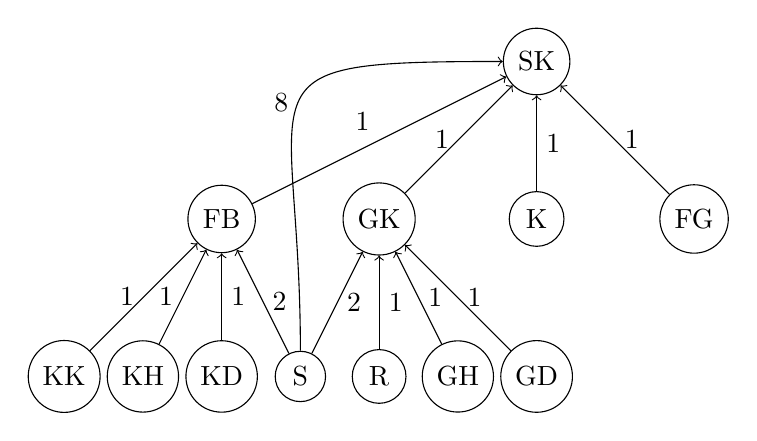
\begin{tikzpicture}
				\node[circle,draw=black, fill=white] (SK) at (0,0) {SK};
				
				\node[circle,draw=black, fill=white] (FB) at (-4,-2) {FB};
				\node[circle,draw=black, fill=white] (GK) at (-2,-2) {GK};
				\node[circle,draw=black, fill=white] (K) at (0,-2) {K};
				\node[circle,draw=black, fill=white] (FG) at (2,-2) {FG};
				
				\node[circle,draw=black, fill=white] (KK) at (-6,-4) {KK};
				\node[circle,draw=black, fill=white] (KH) at (-5,-4) {KH};
				\node[circle,draw=black, fill=white] (KD) at (-4,-4) {KD};
				\node[circle,draw=black, fill=white] (S2) at (-3,-4) {S};
				\node[circle,draw=black, fill=white] (R) at (-2,-4) {R};
				\node[circle,draw=black, fill=white] (GH) at (-1,-4) {GH};
				\node[circle,draw=black, fill=white] (GD) at (0,-4) {GD};
				
				\draw[->] (FB) to node[above left] {1} (SK);
				\draw[->] (GK) to node[left] {1} (SK);
				\draw[->] (K) to node[right] {1} (SK);
				\draw[->] (FG) to node[right] {1} (SK);
				
				\draw[->] (KK) to node[left] {1} (FB);
				\draw[->] (KH) to node[left] {1} (FB);
				\draw[->] (KD) to node[right] {1} (FB);
				\draw[->] (S2) to node[right] {2} (FB);
				\draw[->] (S2) to node[right] {2} (GK);
				\draw[->] (S2) to[out=90,in=180,looseness=2] node[left] {8} (SK);
				
				\draw[->] (R) to node[right] {1} (GK);
				\draw[->] (GH) to node[right] {1} (GK);
				\draw[->] (GD) to node[right] {1} (GK);
			\end{tikzpicture}
		\end{center}
		\item Für einen Smoker werden $2\cdot 1 + 8 + 2\cdot 1 = 12$ Schrauben benötigt. Also werden für 100 Smoker 120 Schrauben benötigt.
	\end{enumerate}

	\section*{Aufgabe 21}
	\begin{enumerate}[label=(\alph*)]
		\item Es ergibt sich
		\begin{center}
			\begin{tabular}{c|rr|rr}
				\textbf{Teil} & \textbf{Preis} & \textbf{Menge} & \textbf{Wert} & \textbf{Anteil am Gesamtwert} \\
				\hline
				1 & 10,00 \EUR & 8.500 & 85.000,00 \EUR & 3,78 \% \\
 				2 & 80,00 \EUR & 2.000 & 160.000,00 \EUR & 7,12 \% \\
				3 & 600,00 \EUR & 1.500 & 900.000,00 \EUR & 40,05 \% \\
				4 & 1.000,00 \EUR & 300 & 300.000,00 \EUR & 13,35 \% \\
				5 & 9,00 \EUR & 100 & 900,00 \EUR & 0,04 \% \\
				6 & 920,00 \EUR & 45 & 41.400,00 \EUR & 1,84 \% \\
				7 & 500,00 \EUR & 100 & 50.000,00 \EUR & 2,22 \% \\
				8 & 500,00 \EUR & 1.200 & 600.000,00 \EUR & 26,70 \% \\
				9 & 5,00 \EUR & 10.000 & 50.000,00 \EUR & 2,22 \% \\
				10 & 20,00 \EUR & 3.000 & 60.000,00 \EUR & 2,67 \% \\
				\hline
				$\Sigma$ & 3.644,00 \EUR & 26.745 & 2.247.300,00 \EUR & 100 \%
			\end{tabular}
		\end{center}
		Sortiert und kumuliert
		\begin{center}
			\begin{tabular}{c|rr|rr|c}
				\textbf{Teil} & \textbf{Wert \%} & \textbf{Wert kumuliert} & \textbf{Menge \%} & \textbf{Menge kumuliert} & \textbf{Einteilung} \\
				\hline
				3 & 40,05 \% & 40,05 \% & 5,61 \% & 5,61 \% & A \\
				8 & 26,70 \% & 66,75 \% & 4,49 \% & 10,10 \% & A \\
				4 & 13,35 \% & 80,10 \% & 1,12 \% & 11,22 \% & A \\
				2 & 7,12 \% & 87,22 \% & 7,48 \% & 18,70 \% & B \\
				1 & 3,78 \% & 91,00 \% & 31,78 \% & 50,48 \% & B \\
				10 & 2,67 \% & 93,67 \% & 11,22 \% & 61,69 \% & B \\
				7 & 2,22 \% & 95,89 \% & 0,37 \% & 62,07 \% & B \\
				9 & 2,22 \% & 98,12 \% & 37,39 \% & 99,46 \% & C \\
				6 & 1,84 \% & 99,96 \% & 0,17 \% & 99,63 \% & C \\
				5 & 0,04 \% & 100,00 \% & 0,37 \% & 100,00 \% & C
			\end{tabular}
		\end{center}
		\item Grafische Darstellung
		\begin{center}
			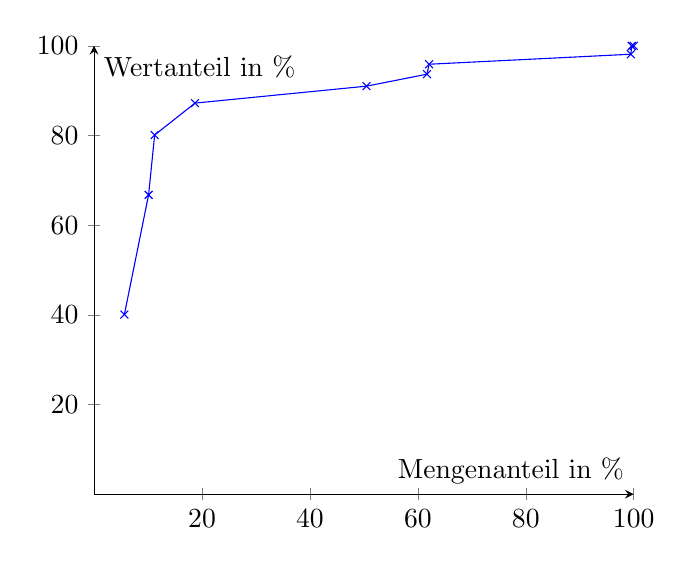
\begin{tikzpicture}
				\begin{axis}[
					xmin=0, xmax=100, xlabel={Mengenanteil in \%},
					ymin=0, ymax=100, ylabel={Wertanteil in \%},
					samples=400,
					axis x line=middle,
					axis y line=middle,
					]
					\addplot[blue,mark=x] coordinates {
						(5.61,40.05)
						(10.10,66.75)
						(11.22,80.10)
						(18.70,87.22)
						(50.48,91)
						(61.69,93.67)
						(62.07,95.89)
						(99.46,98.12)
						(99.63,99.96)
						(100,100)
					};
					
				\end{axis}
			\end{tikzpicture}
		\end{center}
		\item Handlungsweisen für A- und C-Materialien
		\begin{center}
			\begin{longtable}{c|C{5cm}|C{5cm}}
				\textbf{Beschaffungsfunktion} & \textbf{Behandlung der A-Materialien} & \textbf{Behandlung der C-Materialien} \\
				\hline
				Beschaffungmarktforschung & 
				\begin{itemize}[nosep, before=\vspace{-\baselineskip}, after=\vspace{-\baselineskip}, leftmargin=0.3cm]
					\item Intensive Marktanalysen
					\item Beobachtung aller Materialien
					\item Benutzung vieler Informationsquellen
				\end{itemize} & 
				\begin{itemize}[nosep, before=\vspace{-\baselineskip}, after=\vspace{-\baselineskip}, leftmargin=0.3cm]
					\item Starke Beschränkung in den Materialien und Informationsquellen
				\end{itemize} \\
				\hline
				Disposition &
				\begin{itemize}[nosep, before=\vspace{-\baselineskip}, after=\vspace{-\baselineskip}, leftmargin=0.3cm]
					\item Programmorientierte Bedarfsrechnung
					\item Aufwendige Bestellrechnung
					\item Niedrige Sicherheitsbestände
					\item Kurzer Anlieferrhythmus
				\end{itemize} &
				\begin{itemize}[nosep, before=\vspace{-\baselineskip}, after=\vspace{-\baselineskip}, leftmargin=0.3cm]
					\item Verbrauchsorientierte Bedarfsrechnung
					\item Vereinfachte Bestellrechnung
					\item Hohe Sicherheitsbestände
					\item Langer Anlieferrhythmus
				\end{itemize} \\
				\hline
				Bestellabwicklung & 
				\begin{itemize}[nosep, before=\vspace{-\baselineskip}, after=\vspace{-\baselineskip}, leftmargin=0.3cm]
					\item Gründliche Kostenanalysen
					\item Exakte Bedarfsermittlung
					\item Exakte Dispositionsverfahren
					\item Disposition in kurzen Zeitabständen
					\item Strenge Terminkontrolle
					\item Genaue Rechnungsprüfung
					\item Genaue Quantitäts- und Qualitätsprüfung
				\end{itemize} & 
				\begin{itemize}[nosep, before=\vspace{-\baselineskip}, after=\vspace{-\baselineskip}, leftmargin=0.3cm]
					\item Vereinfachte Bestellabwicklung
					\item Automatische Beschaffung in größeren Lagerreichweiten
					\item Wenig aufwendige Terminkontrolle, Rechnungsprüfung, Qualitätsprüfung
					\item Prüfung einer Outsourcing-Entscheidung
				\end{itemize} \\
				\hline
				Bevorratung & 
				\begin{itemize}[nosep, before=\vspace{-\baselineskip}, after=\vspace{-\baselineskip}, leftmargin=0.3cm]
					\item Niedrige Lagerbestände
					\item Kurze Lagerreichweiten
					\item Genaue Festlegung der Sicherheitsbestände
					\item Just-in-Time-Bezug
				\end{itemize} & 
				\begin{itemize}[nosep, before=\vspace{-\baselineskip}, after=\vspace{-\baselineskip}, leftmargin=0.3cm]
					\item Hohe Lagerbestände
				\end{itemize} \\
				\hline
				Wertanalyse & Durchführung & keine Durchführung \\
				\hline
				Inventur & Permanente Inventur & Stichprobeninventur
			\end{longtable}
		\end{center}
	\end{enumerate}
	
	
\end{document}